\section{Emergent Coordination via Shared Vision}
\label{sec:coordination}

This section presents the core contribution of the paper: a set of coordination primitives that let two independent arms cooperatively lift, translate, and lower a tray without any direct communication. All primitives share a common design principle, and are linked by a finite-state protocol (\cref{sec:protocol}) that both arms execute identically.

\subsection{Design Principle: Shared Observation as Shared State}
Much like humans tasked with moving a large object without communicating, two arms can still coordinate if, at every decision point, they have an observable representation of the information they would otherwise need to exchange. Our design uses three such proxies:

\begin{itemize}
  \item \textbf{Tray markers as shared position state.} Both arms see both tray markers. Their positions define what ``the
  tray is here'' means and their height difference defines
  what ``the tray is level'' means, for example.
  \item \textbf{Physical pre-move as a handshake signal.} Instead
  of sending a ``ready to lift'' message in a traditional sense, one arm physically lifts its side of the tray. 
  If the other arm knows to watch for that lift, the message has just been successfully passed.
  \item \textbf{The opposing gripper marker as a position reference
  during motion.} Tray markers are small (20 mm) and frequently
  drop during motion. The gripper markers are large (40 mm)
  and reliably visible. The follower in \cref{sec:translate} tracks
  the leader's gripper rather than the leader's tray marker during periods of faster motion.
\end{itemize}
With this message-passing framework, coordination is now enabled.


\begin{figure} 
    \centering
    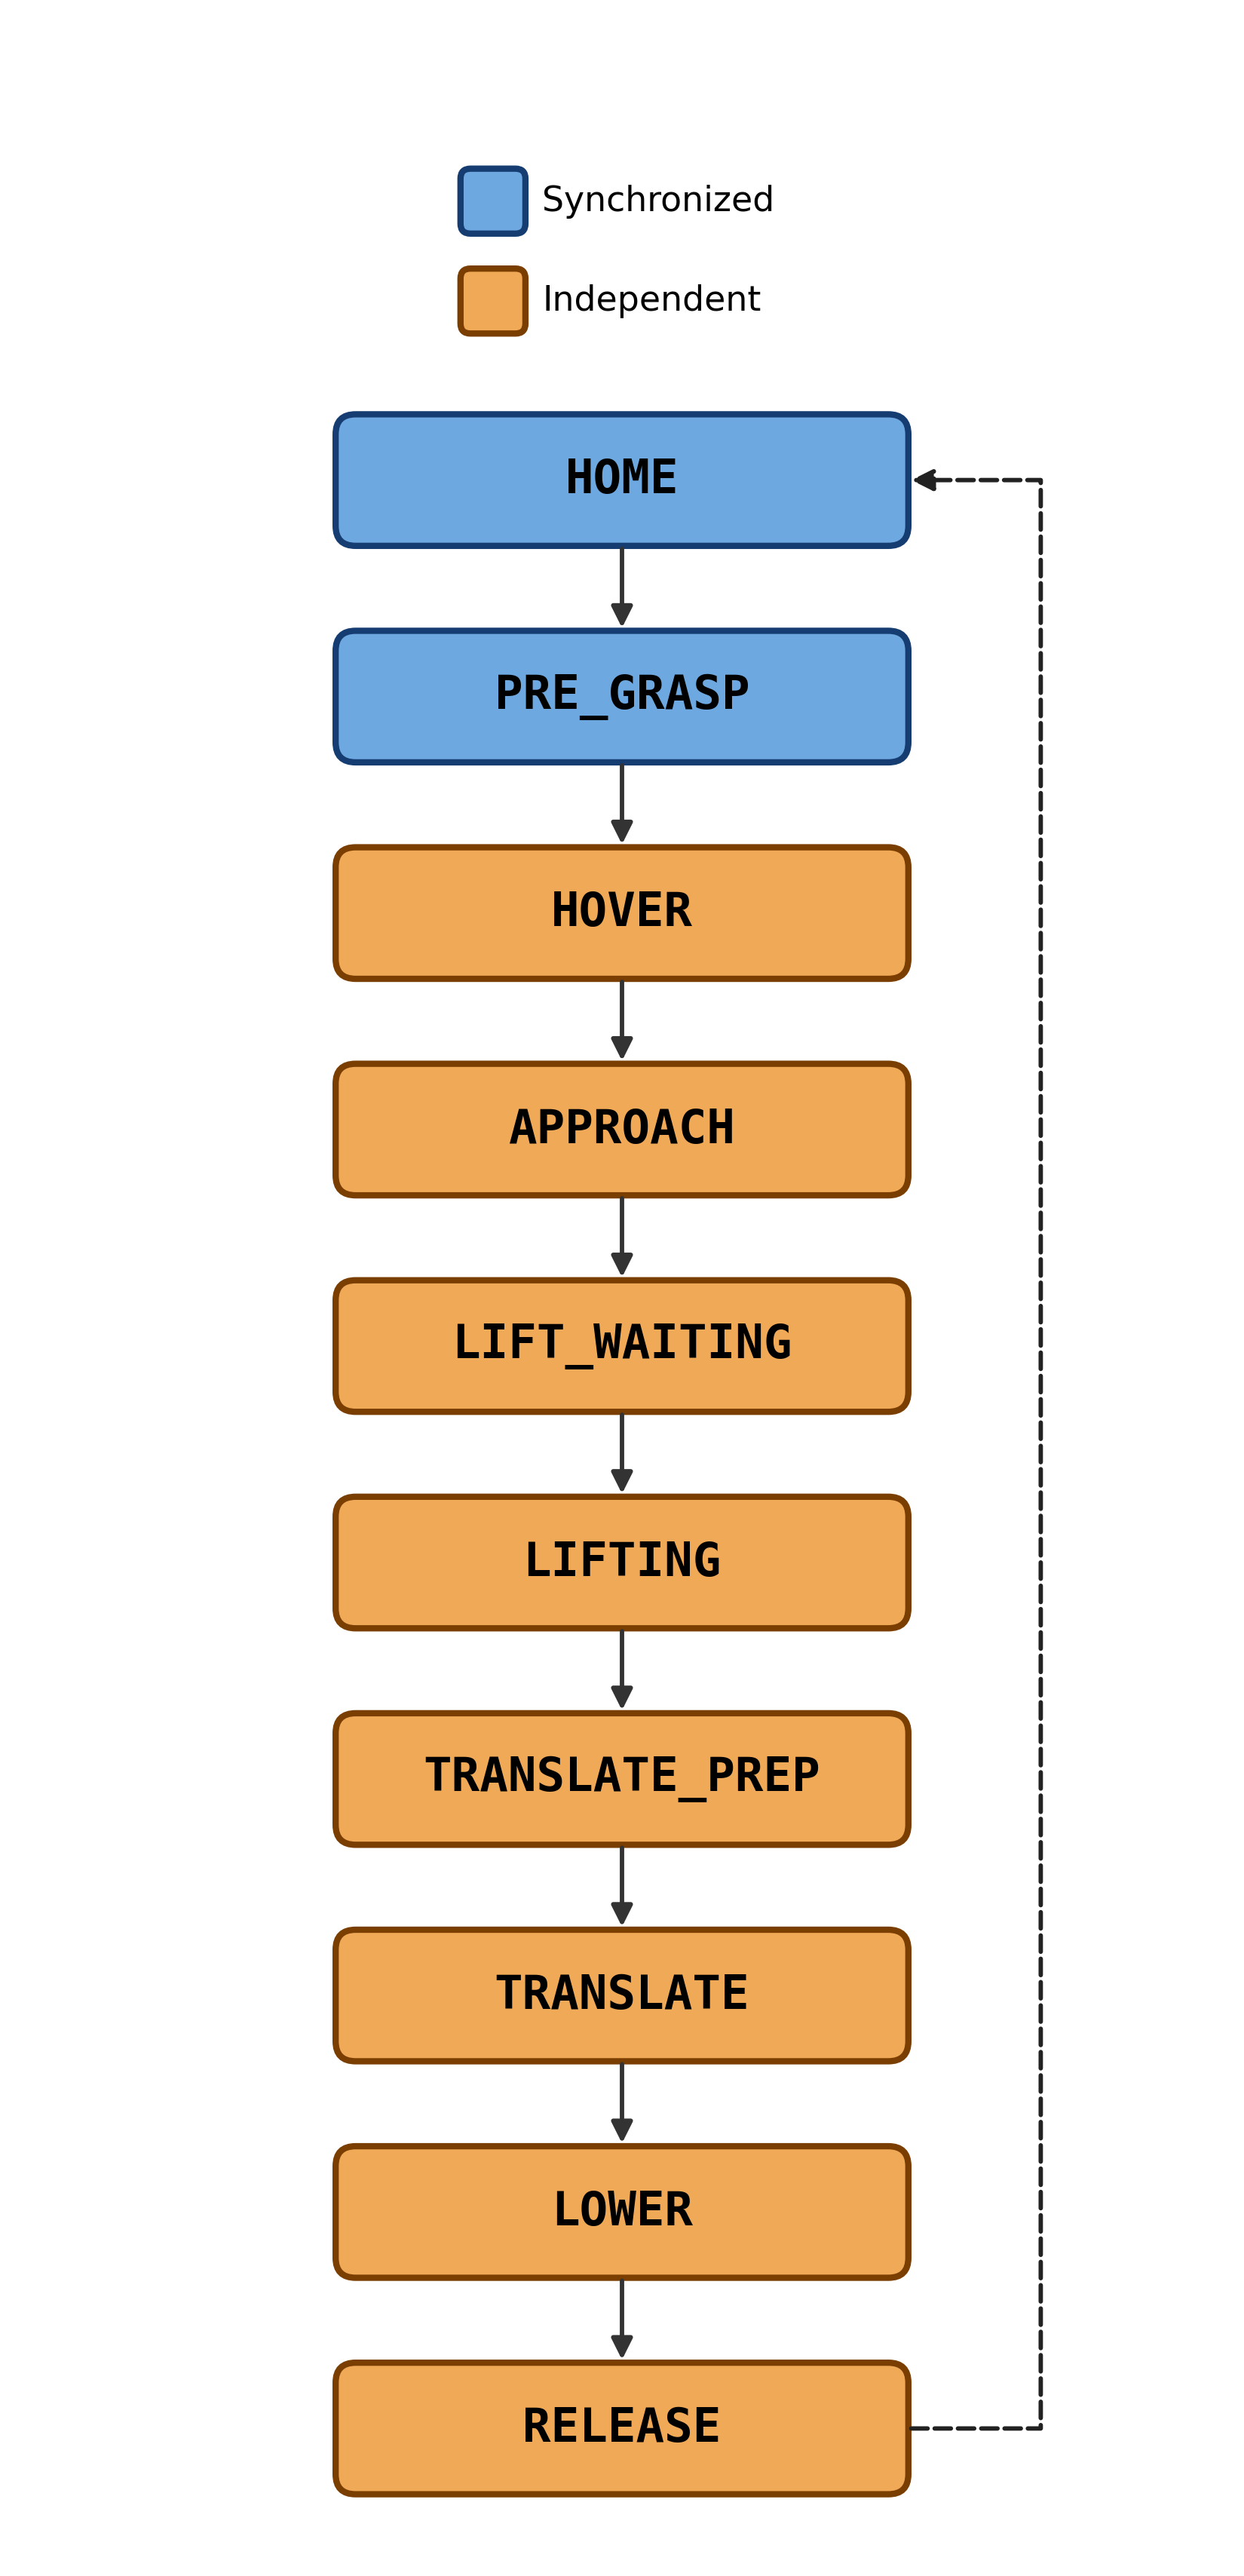
\includegraphics[width=1.16\linewidth]{subtex//images/figure9_state_diagram.png}
    \caption{Shared state-machine run by both arms. All states after \texttt{PRE\_GRASP} run independently. \texttt{PRE\_GRASP} serves only to move the arms into view of the camera, after which coordination must emerge.}
    \label{fig:fsm}
\end{figure}



\subsection{Finite-State Coordination Protocol}
\label{sec:protocol}
Both arms run the linear state machine shown in \cref{fig:fsm}. The first two states (\texttt{HOME} and \texttt{PRE\_GRASP}) are executed by the main thread with synchronized pre-planned moves that bring both arms to the center of the working area. From the \texttt{HOVER} phase onward, each arm runs the state machine in its own thread, issues its own commands, and transitions on its own visual events. The subsequent sections will detail each state and how the transitions to the next state are decided.


\subsection{Hover Convergence}
\label{sec:hover}
\cref{algo:hover} is the controller each arm runs during the
\texttt{HOVER} state. The arm servos over its own tray marker
through its motion map, with the gripper-to-target error fed back into the polynomial query as in \cref{sec:motionmap}. A transient raise proportional to $\|\vec{e}\|$ keeps the gripper \emph{above} the tray as it converges; a 30\% descent bias (subtracting $0.3\,\Delta_{\text{descent}}$ from the polynomial output) keeps the arm slightly above hover height when $\|\vec{e}\|\!\to\!0$, so the arm doesn't come into contact with the tray until it is time to grab. Importantly, the camera readings are converted into the base frame of each
arm first, as both motion maps work in that frame to allow generalization to new environments. A second note is that every position written to the servos is clamped under a maximum delta to decrease hardware stress.

\begin{algorithm} [h]
\caption{HOVER controller}
\label{algo:hover}
\begin{algorithmic}[1]
  \REQUIRE motion map $M$, my tray marker id, my gripper marker id,
           descent delta $\Delta_d$, base transform
           $T_{\text{base}}^{\text{cam}}$
  \STATE $\bar{\vec{x}} \gets \texttt{None}$;\ \ $n_{\text{conv}} \gets 0$
  \LOOP
    \STATE $F \gets \texttt{get\_frame}()$;\ \
           poses $\gets \texttt{detect}(F)$
    \STATE $\vec{x}_{\text{tray}}^{\text{cam}} \gets$
           \texttt{tray\_pose}(poses)
    \IF{$\vec{x}_{\text{tray}}^{\text{cam}}$ is \texttt{None}} \textbf{continue}
    \ENDIF
    \STATE $\vec{x}_{\text{tray}} \gets T_{\text{base}}^{\text{cam}}
           {\vec{x}}_{\text{tray}}^{\text{cam}}$
           \COMMENT{base frame transform}
    \STATE $\bar{\vec{x}} \gets
           \alpha\,\vec{x}_{\text{tray}} + (1\!-\!\alpha)\bar{\vec{x}}$
           \COMMENT{EMA, $\alpha{=}0.2$}
    \STATE $\vec{x}_{\text{tgt}} \gets \bar{\vec{x}} - \vec{o}_{\text{pos}}$
           \COMMENT{bake in position offset}
    \STATE $\vec{x}_{\text{grip}} \gets T_{\text{base}}^{\text{cam}}$\,
           \texttt{gripper\_pose}(poses)
    \STATE $\vec{e} \gets \vec{x}_{\text{tgt}} - \vec{x}_{\text{grip}}$
    \STATE $\vec{q} \gets M(\bar{\vec{x}} + \beta\vec{e})$
           \COMMENT{feedback-corrected query}
    \STATE $\vec{q} \gets \vec{q} - 0.3\,\Delta_d$
           \COMMENT{absolute height increase}
    \STATE $\vec{q} \gets \vec{q} + (\|\vec{e}\|/r_0)\,\vec{\Delta}_{\text{raise}}$
           \COMMENT{error-driven height increase}
    \STATE clip per-step $|\Delta \vec{q}|\le q_{\max}$,\ write $\vec{q}$
    \IF{$\|\vec{e}\| < \tau_c$} 
    $n_{\text{conv}} \mathrel{+}= 1$
            \COMMENT{require 3 frames to break}
    \ELSE\ $n_{\text{conv}} \gets 0$ \ENDIF
    \IF{$n_{\text{conv}} \ge 3$} \textbf{break} \ENDIF
  \ENDLOOP
\end{algorithmic}
\end{algorithm}

An exponential moving average (EMA) with $\alpha{=}0.2$ smooths the tray position to suppress marker jitter. Convergence is declared when $\|\vec{e}\| <
\texttt{CONVERGENCE\_THRESHOLD\_M}=20$\,mm persists for
\texttt{CONVERGENCE\_READINGS}~$=3$ consecutive frames, guarding against a single lucky measurement. This convergence is the trigger that transitions each arm to the next state. In practice, hovering and converging resulted in the largest desyncronization between arms, so regaining that synchronization in the next phases is essential.


\subsection{Approach: Descend Until Vertically Close}
From \texttt{HOVER}, the arm opens its gripper and descends at a fixed rate (\texttt{LIFT\_STEP\_FRACTION}~$=3\%$ of the descent delta every 20 ms), accumulating commanded joint targets rather than applying a delta after each step, which results in movements too small to bypass the servo dead-band. Descent stops when the vertical distance between the tray marker and the gripper marker falls below \texttt{GRASP\_PROXIMITY\_M}~$=86$\,mm, which is the geometric distance between the gripper marker and tray marker when
the gripper just barely reaches the handle. The gripper closes, and the arm transitions to \texttt{LIFT\_WAITING}. This state has no checks for coordination, so any 
timing problems propagating from the hover are still present.

\subsection{Nudge-Lift Handshake}
\label{sec:nudge}
\cref{algo:nudge} describes the nudge-lift, a key coordination move. If either arm lifts alone, the tray tilts and the task fails. If each arm lifts as soon as it arrives, we rely on the previous states to have been synchronized, which almost never happened in practice. The nudge-lift handshake replaces an explicit message with a simple small physical commitment whre each arm pulls its side of the tray upward by \texttt{NUDGE\_FRACTION}$\,\cdot\,\Delta_{\text{descent}}=40\%$ of a descent delta. Each arm then watches the opposite tray
marker and waits for it to have risen by
\texttt{TAG\_RISE\_THRESHOLD\_M}~$=3$\,mm relative to a baseline position captured during \texttt{PRE\_GRASP}. 

Two properties of this algorithm are worth noting. First, the handshake is symmetric in that both arms do the same thing and wait on the same thing. The protocol has no leader-follower role. Second, the handshake cannot false-positive. If one gripper failed to close on the tray, its side of the tray will never move, so neither arm proceeds. This results in a failure
of the goal, but at least the water won't be spilled and the arms will stop. When an arm detects the other arm's perturbation lift (and has already completed it's own lift), it transitions to the next state.


\begin{algorithm} [h]
\caption{Nudge-lift (physical message passing)}
\label{algo:nudge}
\begin{algorithmic}[1]
  \REQUIRE descent delta $\Delta_d$, opposing tray key $k_{\text{other}}$,
           baseline height $y_{\text{other},0}$,
           thresholds $\tau_r=3$\,mm,\ nudge fraction $\eta_n=0.4$
  \STATE Nudge: smooth move, $-\eta_n\Delta_d$ in joint space
  \LOOP
    \STATE $F \gets \texttt{get\_frame}()$;\ poses $\gets \texttt{detect}(F)$
    \STATE $y_{\text{other}} \gets $
           \texttt{tray\_poses}(poses)$[k_{\text{other}}]\,.y$
    \STATE $\texttt{rise} \gets y_{\text{other},0} - y_{\text{other}}$
           \COMMENT{camera $y$ down; rise = $-\Delta y$}
    \IF{$\texttt{rise}\ge \tau_r$} \textbf{break} \ENDIF
  \ENDLOOP
\end{algorithmic}
\end{algorithm}

\subsection{Tilt-Aware Synchronized Lift}
\label{sec:lifting}
Once the handshake completes, both arms transition to \texttt{LIFTING} simultaneously (within one frame of each other, bounded by the rise-detection latency). It is possible that a hard-coded lift would be viable here because the arms are well coordinated at this point, but this poses no merit and a synchronized lift would guarantee success. 


Therefore, we implement coordination as a sort of self-throttling. At each \texttt{LIFTING} step, each arm measures both tray markers' rise from baseline and advances its own target upward only if its own side is lower than the other:
\begin{equation}
\label{eq:lift-gate}
  \text{step this tick} \iff
  (\text{my rise}) \le (\text{other rise}).
\end{equation}
This is a one-line rule with important properties. If the two arms move identically, both step every tick and ascend together. If one arm leads, it stops stepping until the other catches up. If one arm's servos stall transiently, the other naturally pauses. Neither arm ever needs to know which arm is leading. Both arms see the same heights and make the same local decision, and the tray stays level to within the measurement noise. Another important part of this algorithm differentiating it from predecessors is that it uses an explicit sleep for 20 ms every loop. This prevents stacking the same joint delta extremely quickly, as everything in this loop is quick to compute.

Once an arm's own rise reaches \texttt{LIFT\_HEIGHT\_M}~$=60$\,mm, it stops looping and proceeds to \texttt{TRANSLATE\_PREP}. Because the arms are so synchronized during the lift, this transition usually happens at the same time, offset by only a few frames. This culminates in global synchronized from visual cues alone.

\begin{algorithm} [h]
\caption{Tilt-aware LIFTING}
\label{algo:lift}
\begin{algorithmic}[1]
  \REQUIRE per-step lift $\vec{\delta}=-\,\texttt{LIFT\_STEP\_FRACTION}\,\Delta_d$,
           target rise $H$, my tray key $k_m$, other key $k_o$,
           baselines $y_{m,0}, y_{o,0}$
  \STATE $\vec{q}^\star \gets $ \texttt{read\_joints()}
  \LOOP
    \STATE poses $\gets \texttt{detect}(\texttt{get\_frame}())$
    \STATE $r_m \gets y_{m,0}-\text{poses}[k_m].y$;\ \
           $r_o \gets y_{o,0}-\text{poses}[k_o].y$
    \IF{$r_m \ge H$} \textbf{break} 
    \ENDIF
    \IF{$r_m \le r_o$}
       \STATE $\vec{q}^\star \gets \vec{q}^\star + \vec{\delta}$;\ \
              \texttt{write\_joints}($\vec{q}^\star$)
    \ENDIF
    \STATE \texttt{sleep}(20\,ms)
  \ENDLOOP

\end{algorithmic}
\end{algorithm}

\subsection{Leader--Follower Translation}
\label{sec:translate}
The tray is now lifted and level. The forward translation must move both grasp points through the same horizontal trajectory at the same speed, or the tray pivots about whichever point lags. Because the grippers must remain spaced by the tray width, the simplest plan to have both arms sweep an interpolation from the current position to a goal will not work. Coordination is required.

We instead utilize an asymmetric leader-follower scheme. Before
\texttt{TRANSLATE} begins, a single observation measures the
base-frame offset from the left gripper marker to the
right tray marker:
\begin{equation}
\label{eq:offset}
  \vec{o} \;=\; \vec{x}_{\text{tray}_r}^{\text{base}_r}
           - \vec{x}_{\text{grip}_l}^{\text{base}_r},
\end{equation}
where both quantities are expressed in the right arm's base
frame. Because the tray is rigid and level after \cref{algo:lift},
this offset is a constant over the translation. It encodes the
tray width plus whatever small offset the grippers impose.

During translation, the left arm acts as the \textbf{leader}. It plans an interpolation in $(x,z)$ from its current
position to a pre-recorded destination way-point, evaluates its motion map at each intermediate query, and writes to the joints. It is essential that this interpolation happens in 3D space and uses the motion map because the simpler linear interpolation in joint space creates less-intuitive curved trajectories that sometimes resulted in infeasible follower tracking or tray bending. The right arm acts as the \textbf{follower}: each tick, it reads the left gripper marker (large, reliable), transforms it into its own base frame, and adds the offset $\vec{o}$ to obtain its target. Evaluating the right-arm motion map at this target yields the follower's joint command. An EMA ($\alpha=0.1$) smooths the
target to dampen marker noise.

As presented, this algorithm resulted in large jump discontinuities between the top of the lift and the beginning of the (somewhat) smooth slide. To remedy this, we implemented
a \texttt{TRANSLATE\_PREP} phase as mentioned in the previous section. This phase happens immediately after the lift, and consists of only an interpolation between the current position and the first motion map query result in joint space over one second. This serves to smooth the jump from joint space
onto the motion map. After the one second, each arm immediately transitions to \texttt{TRANSLATE}.
Conceptually, this phase should not be necessary, but in practice we concluded that our implementation of
\texttt{find\_closest\_coords}, a brute-force motion map method that finds coordinates nearby to the inputted joint positions by checking error at all of the points, results in jumps that are larger than we had hoped. Our hypothesis is that because we are finding nearby points in joint space, the nearest point might be something that is a close match for a few of the motors, resulting in low error, but far for one or two of the motors causing a large swing. \texttt{TRANSLATE\_PREP} solves this issue.

The key observation coordination-wise is that the follower never needs to know the leader's plan. Whatever trajectory the leader executes, the follower tracks it through
$\vec{o}$, because the leader's gripper position encodes its
intent with zero latency via the shared camera. The full algorithm is presented in \cref{algo:translate}.

\begin{algorithm} [h]
\caption{TRANSLATE: leader and follower}
\label{algo:translate}
\begin{algorithmic}[1]
  \STATE {\bfseries Pre:} measure
         $\vec{o} \gets \vec{x}_{\text{tray}_r} -
          \vec{x}_{\text{grip}_l}$ once
  \STATE // \emph{Leader (side = left):}
  \STATE $\vec{x}_s \gets$ current tray $(x,z)$
  \STATE $\vec{x}_d \gets$ \texttt{find\_closest\_coords}($M_l$,
         way-point$_{\text{left}}$)
  \FOR{$k=1,\dots,n_{\text{steps}}$}
    \STATE $\vec{x}_k \gets \vec{x}_s + smooth(\vec{x}_d-\vec{x}_s)$
    \STATE $\vec{q} \gets M_l(\vec{x}_k) + \vec{h}_{\text{trim}}$;\
           \texttt{write\_joints}($\vec{q}$)
    \STATE \texttt{sleep}(33\,ms)
  \ENDFOR
  \STATE // \emph{Follower (side = right):}
  \FOR{$k=1,\dots,n_{\text{steps}}$}
    \STATE $\vec{x}_g \gets T_{\text{base}_r}^{\text{cam}}\,
           \texttt{gripper\_pose}_\text{left}(\text{poses})$
    \STATE $\vec{x}_t \gets \vec{x}_g + \vec{o}$
    \STATE $\bar{\vec{x}}_t \gets
           \alpha_f\vec{x}_t+(1\!-\!\alpha_f)\bar{\vec{x}}_t$
           \COMMENT{EMA, $\alpha_f{=}0.1$}
    \STATE $\vec{q} \gets M_r(\bar{\vec{x}}_t) + \vec{h}_{\text{trim}}$;
           \ \texttt{write\_joints}($\vec{q}$)
    \STATE \texttt{sleep}(33\,ms)
  \ENDFOR
\end{algorithmic}
\end{algorithm}

\subsection{Tilt-Aware Lowering}
\label{sec:lower}
Lowering is mostly symmetric to the lift, and has similar failure modes, but the motion is opposite. We protect against the tilting failures with a tilt-pause rule (\cref{algo:lower}): at each tick, the arm pauses its descent if
its own tray marker is physically lower than the other's by more
than \texttt{TILT\_PAUSE\_THRESHOLD\_M}~$=5$\,mm, letting the
higher side catch up before both sides continue down. The rule is identical on both arms which, like \eqref{eq:lift-gate}, naturally synchronizes two independent descenders. One thing to note about this algorithm is the use of a discrete counter variable to limit how long the loop can run for. This is because we need to guarantee that both arms will eventually release the tray to finish the movement. This remedies an issue
in which the arms would lower the tray to the table, but continue to hold it waiting to lower further. The parameter was tuned such that the arms never let go of the tray too early.

\begin{algorithm} [t]
\caption{Tilt-aware LOWER}
\label{algo:lower}
\begin{algorithmic}[1]
  \REQUIRE lower destination $\vec{q}_d$, duration $T$,
           threshold $\tau_t=5$\,mm
  \STATE $\vec{q}_s \gets$ \texttt{read\_joints()};\ \ $k \gets 0$
  \WHILE{$k < n$}
    \STATE poses $\gets \texttt{detect}(\texttt{get\_frame}())$
    \STATE $\texttt{tilt} \gets
            \text{poses}[k_m].y - \text{poses}[k_o].y$
            \COMMENT{cam $y$ down}
    \IF{$\texttt{tilt} > \tau_t$}
      \STATE // my side lower: wait
      \STATE \texttt{sleep}(20\,ms);\ \textbf{continue}
    \ENDIF
    \STATE $\vec{q} \gets \vec{q}_s + smooth(\vec{q}_d-\vec{q}_s)$;
           \ \texttt{write\_joints}($\vec{q}$)
    \STATE $k \gets k+1$;\ \texttt{sleep}(20\,ms)
  \ENDWHILE
\end{algorithmic}
\end{algorithm}

\subsection{Release and Return}
On \texttt{RELEASE}, each arm opens its gripper and performs an interpolated move to a pre-recorded way-point that is directly above the tray to ensure clearance, then to the home way-point. No coordination is required here as the tray is static on the table. Now the task has been completed.
